\documentclass[11pt,letterpaper]{article}
\usepackage[utf8]{inputenc}

%----- Configuración del estilo del documento------%
\usepackage{epsfig,graphicx}
\usepackage[left=2cm,right=2cm,top=1.8cm,bottom=2.3cm]{geometry}
\usepackage{fancyhdr}
\usepackage{lastpage}

\usepackage{xcolor}
\usepackage{soul}
\newcommand{\mathcolorbox}[2]{\colorbox{#1}{$\displaystyle #2$}}

%Color bibi
\definecolor{bibi}{RGB}{0,103,148}
% Otros colores

%------ Paquetes de dibujo --------%
\usepackage{tikz}
\usepackage{circuitikz}

%------ Paquetes para mantener las imágenes en su lugar --------%
\usepackage{float}

%------ Paquete para notacion de dirac -------%
\usepackage{braket}

%------ Paquetes para mantener las imágenes en su lugar --------%
\usepackage{float}

%------ Paquete para codigo 
\usepackage{minted}

\usepackage{cite}
\usepackage{multicol}
\setlength{\columnsep}{1.5cm}
\setlength{\columnseprule}{.5pt}

\pagestyle{fancy}
\fancyhf{}
\rfoot{\textit{Página \thepage \hspace{1pt} de \pageref{LastPage}}}

%------ Paquetes matemáticos básicos --------%
\usepackage{amsmath}
\usepackage{amssymb}
\usepackage{amsthm}

\begin{document}
%------ Encabezado -------- %
\begin{center}
    \begin{minipage}{3cm}
    	\begin{center}
    		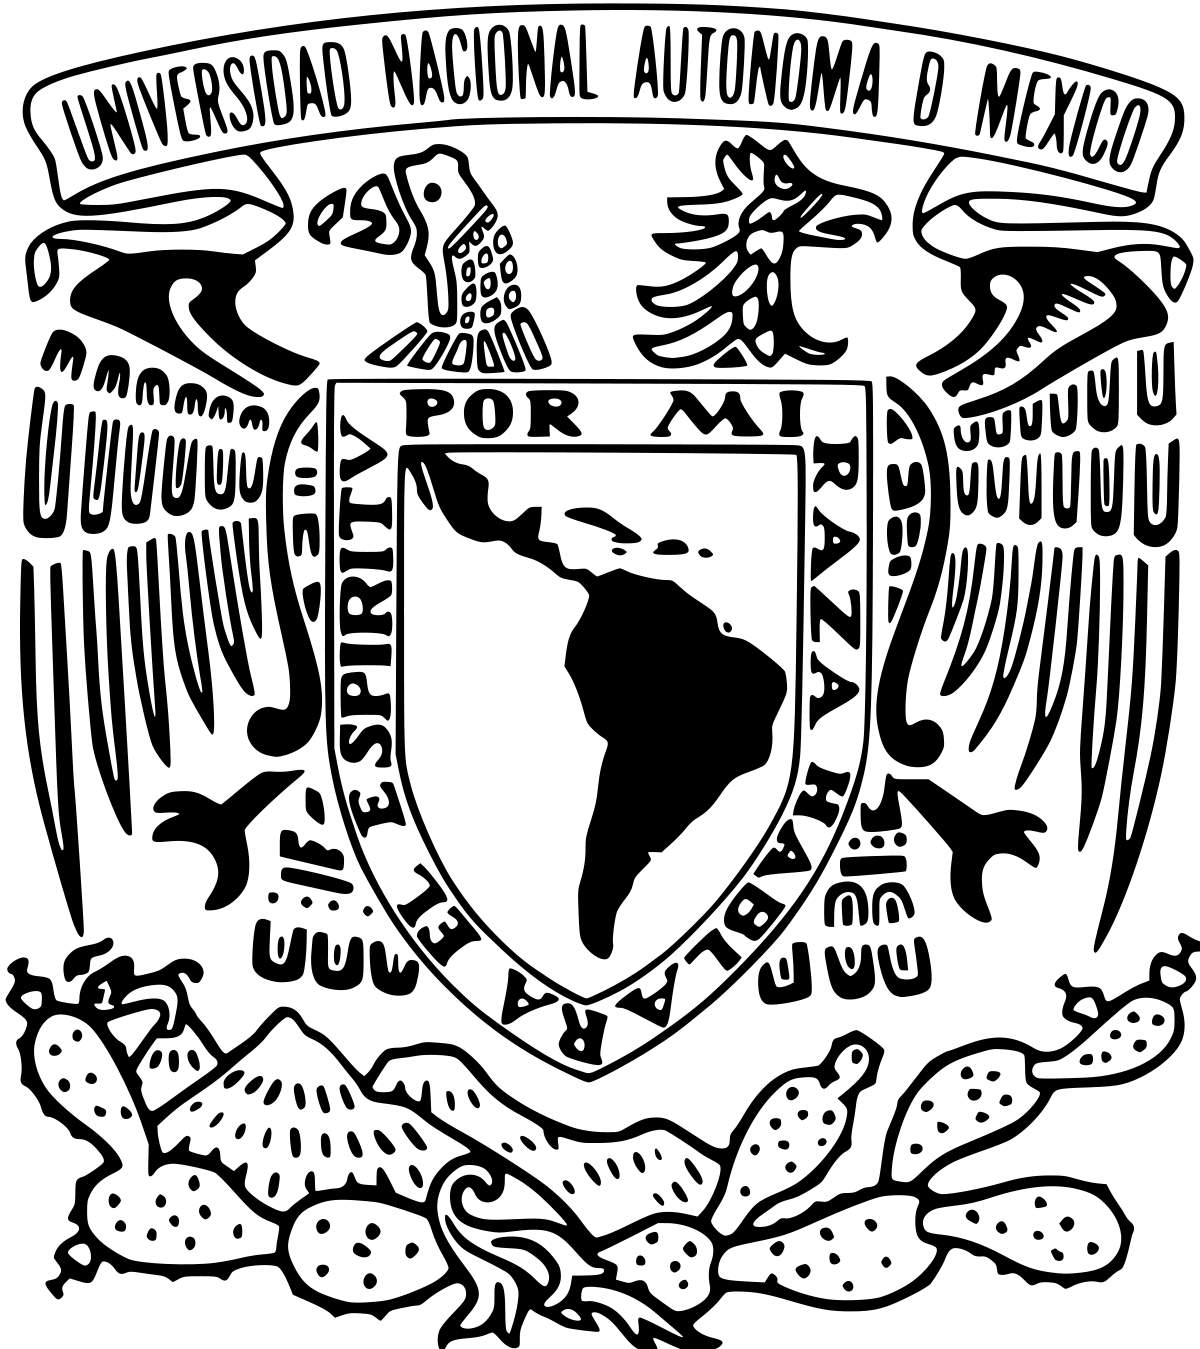
\includegraphics[height=3.3cm]{src/Img/Logo_UNAM.png}
    	\end{center}
    \end{minipage}\hfill
    \begin{minipage}{10cm}
    	\begin{center}
    	\textbf{\large Universidad Nacional Autónoma de México}\\[0.1cm]
        \textbf{Facultad de Ciencias}\\[0.1cm]
        \textbf{Criptografía y seguridad $|$ 7133}\\[0.1cm]
        Tarea corta 2 : $|$ Divisibilidad 9 \\[0.1cm]
        Sosa Romo Juan Mario $|$ 320051926 \\[0.1cm]
        16/09/24
    	\end{center}
    \end{minipage}\hfill
    \begin{minipage}{3cm}
    	\begin{center}
    		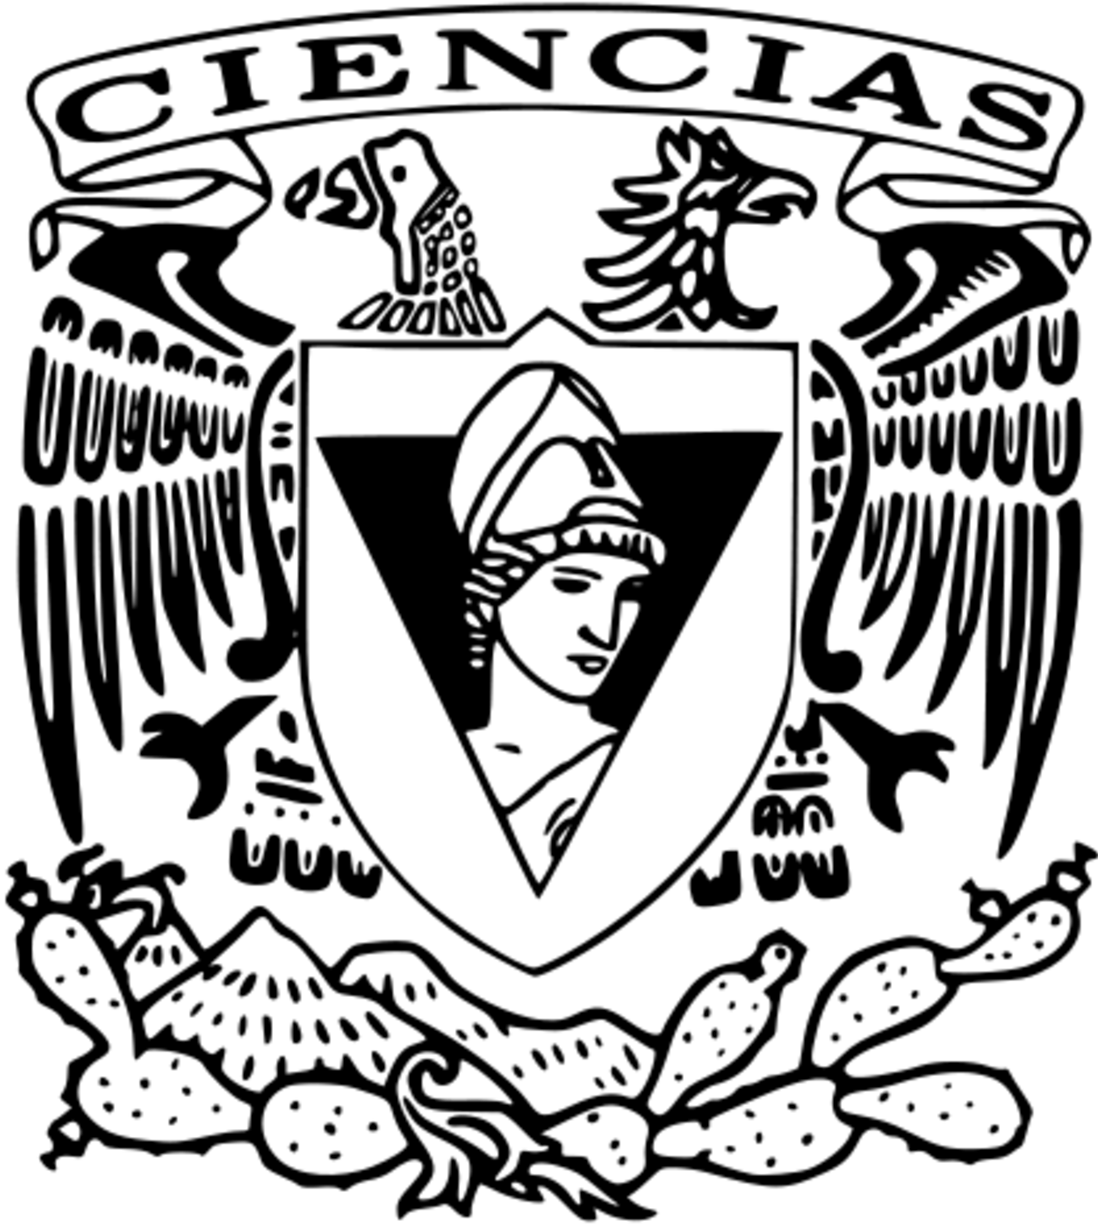
\includegraphics[height=3.3cm]{src/Img/Logo_FC.png}
    	\end{center}
    \end{minipage}
\end{center}


\rule{16.99cm}{0.1mm}

%------ Ejercicios -------- %
\begin{enumerate}
    \item \textbf{Descifrar el archivo file1.lol}
\begin{quote}
    Para el archivo \texttt{file1.lol} se comenzó inspeccionando su contenido binario en bruto,
    mostrando tanto los primeros caracteres en ASCII como en hexadecimal. El resultado
    no presentaba texto legible, sino bytes aparentemente aleatorios, lo que sugirió que se
    trataba de un cifrado clásico sobre bytes y no de una simple codificación.

    A continuación, se implementó un procedimiento en Python para probar de manera
    automática los cifrados César, Decimado y Afín, utilizando fuerza bruta sobre todas sus
    posibles claves. Una vez obtenido cada descifrado, se verificaba la cabecera con los
    \textit{magic bytes} característicos de distintos formatos (PDF, PNG, MP3, MP4).

    Para el caso del cifrado Afín, se utilizó la siguiente función que aplica la fórmula de
    descifrado con aritmética modular en $Z_{256}$:

    \vspace{.3cm}
    \begin{verbatim}
    def affine_decrypt(data, a, b):
        try:
            inv = pow(a, -1, 256)  # inverso modular de a
        except ValueError:
            return None
    
        result = bytearray()
        for byte in data:
            val = ((byte - b) * inv) % 256
            result.append(val)
        return result
    \end{verbatim}
    \vspace{.3cm}
    
    Tras las pruebas, se encontró que el método correcto era el \textbf{cifrado Afín} con
    parámetros $a=143$ y $b=157$. El archivo resultante comenzaba con la secuencia
    \texttt{0xFF 0xFB}, correspondiente al \textit{frame sync} de los archivos de audio MPEG
    Layer III (\texttt{.mp3}), lo que confirmó el formato.

    Una vez guardado el archivo descifrado, se verificó que podía reproducirse
    correctamente como audio. Con esto se validó el éxito del proceso de descifrado.
\end{quote}
\vspace{.5cm}

    \begin{enumerate}
        \item \textbf{}\vspace{.2cm}
\textcolor{bibi}{}
\begin{quote}
\end{quote}
        \item \textbf{}\vspace{.2cm}
\textcolor{bibi}{}
\begin{quote}
\end{quote}
        \item \textbf{}\vspace{.2cm}
\textcolor{bibi}{}
\begin{quote}
\end{quote}
        \item \textbf{}\vspace{.2cm}
\textcolor{bibi}{}
\begin{quote}
\end{quote}
    \end{enumerate}
    \item \textbf{Ataque}

    \item \textbf{Descifrar el archivo file3.lol}

\begin{quote}
    Comencé por inspeccionar un poco el archivo utilizando un poco de código de Python:
    \vspace{.3cm}

    \begin{minted}[fontsize=\small, linenos, frame=single]{python}
def ascii_preview(b, length=512):
  s = b[:length]
  txt = ''.join(chr(x) if 32 <= x < 127 or x in (9,10,13) else '.' for x in s)
  return txt

print("=== ASCII preview")
print(ascii_preview(head, 512))
print("\n=== Hex ===")
print(' '.join(f"{x:02x}" for x in head[:128]))
    \end{minted}
    \vspace{.3cm}

    Como nota, todo el código que voy a mostrar para este procedimiento está incluido en el \texttt{p1CriptoEj3.ipynb} dentro del \texttt{src}.

    \begin{center}
    	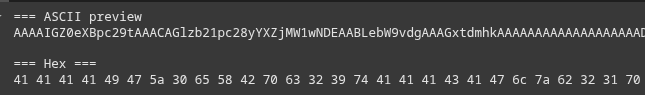
\includegraphics[width=.9\textwidth]{resources/ej3.png} 
    \end{center}

    De aquí, consulte con diversos LLMs para que me resaltaran el hecho de que todos los
    caracteres que encontré son imprimibles pertenecientes al alfabeto Base64 por lo que hice
    algunos tests para ver si se trataba de esta codificación. \vspace{.3cm}

    \begin{minted}[fontsize=\small, linenos, frame=single]{python}
# 1) bytes del head en base 64
only_b64 = all((c in B64_CHARS_WITH_NL) for c in head)
print("\n1) Bytes de head en b64?", only_b64)

# 2) padding con =
has_eq = b'=' in raw[-16:] or b'=\n' in raw or raw.rstrip().endswith(b'=')
print("2) Padding con =:", has_eq)

# 3) contar caracteres en ASCII
visible_chars = [c for c in head if 32 <= c < 127 or c in (9,10,13)]
if visible_chars:
    b64_count = sum(1 for c in visible_chars if c in B64_STD or c in (10,13))
    frac = b64_count / len(visible_chars)
else:
    frac = 0.0
print(f"3) Fraccion de contenido que es ASCII: {frac:.3f}")

# 4) Medir porcentaje de lineas longitud 4
lines = ascii_preview(raw, 4096).splitlines()
if lines:
    lengths = [len(l) for l in lines if len(l.strip())>0]
    if lengths:
        multiples_of_4 = sum(1 for L in lengths if L % 4 == 0)
        pct_mult4 = multiples_of_4 / len(lengths)
    else:
        pct_mult4 = 0.0
else:
    pct_mult4 = 0.0
print(f"4) Medir porcentaje de lineas longitud 4: {pct_mult4:.3f}")

# 5) Buscar firmas de formatos binarios
signs = []
if raw.startswith(b"%PDF"):
    signs.append("PDF")
if raw.startswith(b"\x89PNG\r\n\x1a\n"):
    signs.append("PNG")
if raw.startswith(b"\xff\xd8\xff"):
    signs.append("JPEG")
if raw.startswith(b"PK\x03\x04"):
    signs.append("ZIP")
print("5) Firmas de formatos binarios en el inicio:", signs if signs else "False")
    \end{minted}
    \vspace{.3cm}

    Dandome el siguiente resultado:
    \begin{center}
    	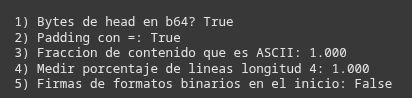
\includegraphics[width=.9\textwidth]{resources/ej3.2.png} 
    \end{center}

    Por estas métricas, todo indica que es base64. Como breviario cultural, la base 64 es una
    forma de codificar binario en texto de manera que los datos binarios están
    representados en secuencias de caracteres imprimibles usando el formato ASCII,
    específicamente cada 6 bits de los datos binarios de representan con un carácter del
    conjunto de 64 posibles. Es útil para transmitir datos binarios si solo podemos poner
    texto ademas, si la cadena no es del tamaño adecuado se utiliza el carácter de relleno $=$.
    Vemos que de las métricas recolectadas, todo parece apuntar a esta codificación.
    \vspace{.3cm}

    Hice un código que verifica con heurísticas si es base 64, e implemente una
    decodificación de base64, después busca en la cabeza del nuevo archivo los magic bytes para
    saber la extensión del archivo y después de saber que es \texttt{mp4} puse también
    código para poder verlo en el mismo notebook. Todo esto se puede ver en la ruta antes
    mencionada y aquí los resultados:

    \begin{center}
    	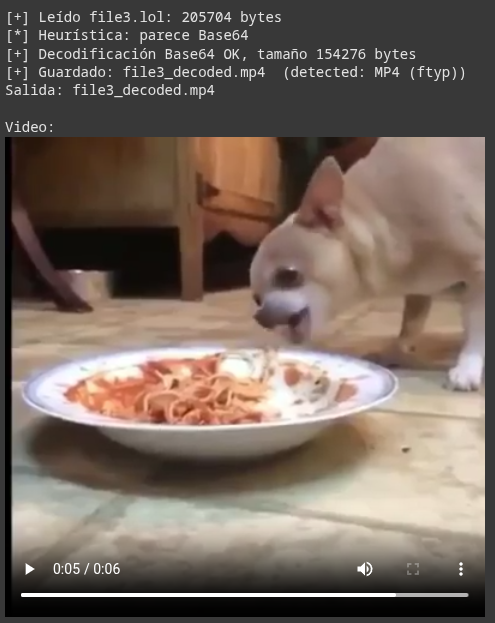
\includegraphics[height=12cm]{resources/ej3.3.png} 
    \end{center}

    Incluyo aquí también el decodificador: \vspace{.3cm}

    \begin{minted}[fontsize=\small, linenos, frame=single]{python}
def base64_decode_from_scratch(s):
  """
  Decodificador base64 desde cero.
  Acepta s como str (puede contener espacios/newlines).
  Devuelve bytes decodificados.
  """
  # Mantener solo chars válidos + '='
  s = ''.join(ch for ch in s if ch in _b64chars or ch == '=')
  if not s:
      return b''
  # Si la longitud no es múltiplo de 4, rellenar con '='
  pad_len = (4 - (len(s) % 4)) % 4
  if pad_len:
      s += '=' * pad_len

  out = bytearray()
  for i in range(0, len(s), 4):
      block = s[i:i+4]
      vals = []
      pad = 0
      for ch in block:
          if ch == '=':
              vals.append(0)
              pad += 1
          else:
              # Asumir 'A' (valor 0) si char inválido
              vals.append(_b64rev.get(ch, 0))
      # recomponer 24 bits
      triple = (vals[0] << 18) | (vals[1] << 12) | (vals[2] << 6) | (vals[3])
      b1 = (triple >> 16) & 0xFF
      b2 = (triple >> 8) & 0xFF
      b3 = triple & 0xFF
      out.append(b1)
      if pad < 2:
          out.append(b2)
      if pad == 0:
          out.append(b3)
  return bytes(out)
    \end{minted}
    \vspace{.3cm}
\end{quote} 
\vspace{.5cm}

    \item \textbf{Dentro de la red}

    \item \textbf{}\vspace{.2cm}
\textcolor{bibi}{}
\begin{quote}
\end{quote}
    \item \textbf{}\vspace{.2cm}
\textcolor{bibi}{}
\begin{quote}
\end{quote}
    \item \textbf{}\vspace{.2cm}
\textcolor{bibi}{}
\begin{quote}
\end{quote}
    \begin{enumerate}
        \item \textbf{}\vspace{.2cm}
\textcolor{bibi}{}
\begin{quote}
\end{quote}
        \item \textbf{}\vspace{.2cm}
\textcolor{bibi}{}
\begin{quote}
\end{quote}
    \end{enumerate}
    \item \textbf{}\vspace{.2cm}
\textcolor{bibi}{}
\begin{quote}
\end{quote}
    \begin{enumerate}
        \item \textbf{}\vspace{.2cm}
\textcolor{bibi}{}
\begin{quote}
\end{quote}
        \item \textbf{}\vspace{.2cm}
\textcolor{bibi}{}
\begin{quote}
\end{quote}

    \end{enumerate}
    \item \textbf{}\vspace{.2cm}
\textcolor{bibi}{}
\begin{quote}
\end{quote}
    \item \textbf{Esto es una prueba uwu}\vspace{.2cm}
\textcolor{bibi}{}
\begin{quote}
	\begin{align*}
		bla
	\end{align*}
\end{quote}

\end{enumerate}

% \textbf{}\vspace{.2cm}
% \textcolor{bibi}{}
% \begin{quote}
% \end{quote}
\begin{align*}
	align*
\end{align*}
\end{document}
